\documentclass[tikz,border=4pt]{standalone}
\usepackage{amsmath,amssymb}
\usepackage{xcolor}
\usetikzlibrary{calc}

\definecolor{gridgray}{RGB}{145,153,160}
\definecolor{edgegray}{RGB}{35,31,32}
\definecolor{faceleft}{RGB}{132,145,201}
\definecolor{facefront}{RGB}{117,133,193}
\definecolor{faceright}{RGB}{100,119,184}
\definecolor{topblue}{RGB}{38,80,162}
\definecolor{wallblue}{RGB}{24,47,171}

\begin{document}
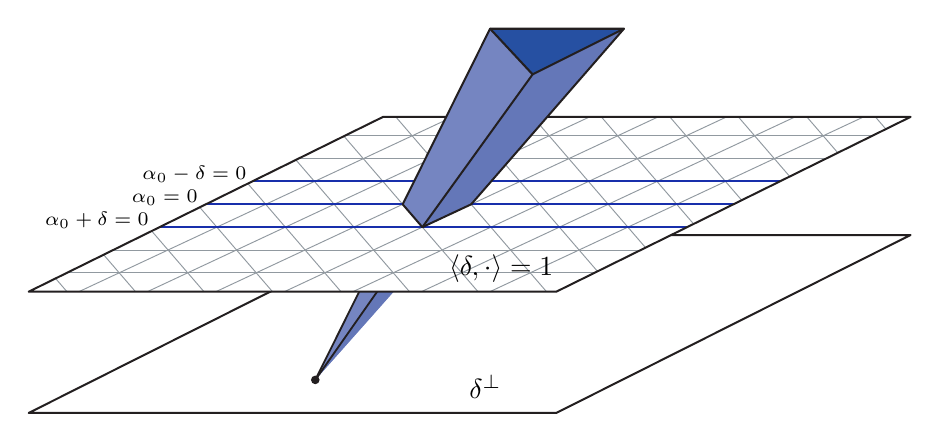
\begin{tikzpicture}[
  x=1cm,
  y=1cm,
  line cap=round,
  line join=round
]

% ============================================================
% Upper affine section
% ============================================================
\coordinate (UFL) at (0.20,2.20);
\coordinate (UFR) at (6.90,2.20);
\coordinate (UBR) at (11.40,4.42);
\coordinate (UBL) at (4.70,4.42);

% ============================================================
% Lower affine section
% ============================================================
\coordinate (LFL) at (0.20,0.66);
\coordinate (LFR) at (6.90,0.66);
\coordinate (LBR) at (11.40,2.92);
\coordinate (LBL) at (4.70,2.92);

% ============================================================
% Cone points
% ============================================================
\coordinate (O) at (3.84,1.08);

% Intersection triangle with the upper plane
\coordinate (A) at (4.95,3.31);
\coordinate (B) at (5.20,3.02);
\coordinate (C) at (5.82,3.31);

% Upper triangular section
\coordinate (Tleft)  at (6.06,5.54);
\coordinate (Tmid)   at (6.60,4.96);
\coordinate (Tright) at (7.76,5.54);

% ============================================================
% 1. Lower plane
% ============================================================
\path[fill=white]
  (LFL)--(LFR)--(LBR)--(LBL)--cycle;

\draw[edgegray,line width=.72pt]
  (LFL)--(LFR)--(LBR)--(LBL)--cycle;

% ============================================================
% 2. Cone below the upper plane
%
% Drawn first, so that the opaque upper plane covers it.
% ============================================================
\path[fill=faceleft,draw=none]
  (O)--(C)--(A)--cycle;

\path[fill=faceright,draw=none]
  (O)--(B)--(C)--cycle;

\path[fill=facefront,draw=none]
  (O)--(A)--(B)--cycle;

% Only visible lower edges
\draw[edgegray,line width=.66pt]
  (O)--(A);

\draw[edgegray,line width=.66pt]
  (O)--(B);

% ============================================================
% 3. Upper plane and triangular grid
% ============================================================
\path[fill=white]
  (UFL)--(UFR)--(UBR)--(UBL)--cycle;

\begin{scope}
  \clip (UFL)--(UFR)--(UBR)--(UBL)--cycle;

  % Local coordinates of the triangular grid
  \begin{scope}[
    shift={(-0.39,2.44)},
    x={(0.87cm,0cm)},
    y={(0.62cm,0.29cm)}
  ]

    % --------------------------------------------------------
    % Three families of grid lines
    % --------------------------------------------------------
    \foreach \j in {-2,...,9}{
      \draw[gridgray,line width=.34pt]
        (-4,\j)--(15,\j);
    }

    \foreach \i in {-6,...,18}{
      \draw[gridgray,line width=.34pt]
        (\i,-8)--(\i,15);
    }

    \foreach \k in {-10,...,28}{
      \draw[gridgray,line width=.34pt]
        (-8,{\k+8})--(20,{\k-20});
    }

    % --------------------------------------------------------
    % Three highlighted parallel affine walls
    %
    % These are members of the grid family y = constant.
    % The upper line y=3 is parallel to and contains A--C.
    % --------------------------------------------------------
    \draw[wallblue,line width=.72pt]
      (-8,2)--(20,2);

    \draw[wallblue,line width=.72pt]
      (-8,3)--(20,3);

    \draw[wallblue,line width=.72pt]
      (-8,4)--(20,4);

    % --------------------------------------------------------
    % Wall labels: no white background rectangles
    % --------------------------------------------------------
   

  \end{scope}
\end{scope}

% Boundary of the upper plane
\draw[edgegray,line width=.72pt]
  (UFL)--(UFR)--(UBR)--(UBL)--cycle;


% ============================================================
% Labels of the three parallel affine walls
% Place them outside the left side of the upper plane,
% slanted-aligned with the plane edge.
% ============================================================
\begin{scope}[
  shift={(-0.39,2.44)},
  x={(0.87cm,0cm)},
  y={(0.62cm,0.29cm)}
]
  % Same local x-coordinate, different local y-levels.
  % This makes the labels align along a slanted line.
  \node[
    font=\scriptsize,
    anchor=east,
    inner sep=0pt
  ] at (.8,2.3) {$\alpha_0+\delta=0$};

  \node[
    font=\scriptsize,
    anchor=east,
    inner sep=0pt
  ] at (.8,3.3) {$\alpha_0=0$};

  \node[
    font=\scriptsize,
    anchor=east,
    inner sep=0pt
  ] at (.8,4.3) {$\alpha_0-\delta=0$};
\end{scope}

% ============================================================
% 4. Cone above the upper plane
%
% Faces have no automatic outlines, so hidden edges are not
% accidentally drawn.
% ============================================================

% Left face
\path[fill=faceleft,draw=none]
  (A)--(C)--(Tright)--(Tleft)--cycle;

% Front face
\path[fill=facefront,draw=none]
  (A)--(B)--(Tmid)--(Tleft)--cycle;

% Right face
\path[fill=faceright,draw=none]
  (B)--(C)--(Tright)--(Tmid)--cycle;

% Top triangular face
\path[fill=topblue,draw=none]
  (Tleft)--(Tmid)--(Tright)--cycle;

% ============================================================
% Visible cone edges
% ============================================================

% Longitudinal ridges
\draw[edgegray,line width=.72pt]
  (A)--(Tleft);

\draw[edgegray,line width=.72pt]
  (B)--(Tmid);

\draw[edgegray,line width=.72pt]
  (C)--(Tright);

% At the plane section, draw only the two visible front edges.
% The hidden rear edge A--C is deliberately omitted.
\draw[edgegray,line width=.72pt]
  (A)--(B);

\draw[edgegray,line width=.72pt]
  (B)--(C);

% Top triangular boundary
\draw[edgegray,line width=.76pt]
  (Tleft)--(Tmid)--(Tright)--cycle;

% ============================================================
% 5. Delta direction
%
% The dashed line follows the central ray of the cone.
% ============================================================

% Centroid of the upper triangular face
\coordinate (Gtop) at (6.8067,5.3467);

% Extend the central ray slightly beyond the top face
\coordinate (Dtip) at ($(O)!1.16!(Gtop)$);
% Midpoint of Tleft--Tright
\coordinate (Mtop) at ($(Tleft)!0.5!(Tright)$);

% Centroid of the top triangular face
\coordinate (Gtop) at ($(Tmid)!0.666667!(Mtop)$);

% Extend the ray O--Gtop beyond the top face
\coordinate (Dtip) at ($(O)!1.18!(Gtop)$);

% Begin just outside the opaque top face
\coordinate (Dstart) at ($(Gtop)!0.04!(Dtip)$);

% \draw[
%   ->,
%   densely dashed,
%   edgegray,
%   line width=.82pt
% ]
%   (Dstart)--(Dtip)
%   node[above,inner sep=1.5pt] {$\delta$};
% Lower vertex
\fill[edgegray]
  (O) circle[radius=1.55pt];

% Top label
\node[
  anchor=south
]
  at (6.,.72)
  {$\delta^\perp$};

\node[
  anchor=south
]
  at (6.2,2.2)
  {$\langle\delta,\cdot\rangle = 1$};

\end{tikzpicture}
\end{document}